\documentclass[10pt]{book}

% --- KDP 6x9 MIT Bleed: Seite = 6.125" x 9.25" ---
\usepackage[
paperwidth=6.125in,
paperheight=9.25in,
inner=1.125in,   % 1.000" + 0.125"
outer=1.025in,   % 0.900" + 0.125"
top=0.925in,     % 0.800" + 0.125"
bottom=1.125in   % 1.000" + 0.125"
]{geometry}

% --- Pakete ---
\usepackage[pages=all]{background}
\usepackage{graphicx}
\usepackage{ragged2e}
\usepackage{parskip}
\usepackage{tikz}
\usepackage{xcolor}
\usepackage[protrusion=true,expansion=true]{microtype} % besseres Druckbild

\setlength{\parindent}{0pt}

% --- Farben (anpassbar) ---
% \definecolor{coverblue}{HTML}{1E4A66} % z.B. Front-Titel
\definecolor{coveraccent}{HTML}{00B7C2} % Akzent (Titel auf Rückseite)
\definecolor{covertext}{HTML}{E6E6E6}   % Fließtext auf dunklem Grund (sehr helles Grau)

% --- Hintergrundbild (bis zum Rand, inkl. Bleed) ---
% Ideal: 300 dpi bei 6.125"x9.25" (~1838x2775 px)
\backgroundsetup{
	scale=1, angle=0, opacity=1,
	contents={
\includegraphics[width=\paperwidth,height=\paperheight]{lichtspuren.png}}
}

\begin{document}
	\thispagestyle{empty}\pagestyle{empty}
	
	% --- dezente Dunkelblende hinter dem Textblock für sichere Lesbarkeit ---
	% Bereich grob: obere Text-Hälfte; Koordinaten bei Bedarf anpassen
	
\begin{tikzpicture}[remember picture,overlay]
		\fill[black,opacity=0.35]
		([xshift=0.45in,yshift=7.9in]current page.south west) rectangle
		([xshift=-0.45in,yshift=3.25in]current page.north east);
	\end{tikzpicture}
	
	% --- Textblock ---
	{\color{coveraccent}\Large\bfseries Photon – Theorie und Anwendungen}\par
	\vspace{-0.3em}
	
	{\color{covertext}
		\linespread{1.08}\selectfont
		\justifying
		\sffamily % moderner Look (entfernen, wenn Serifenschrift gewünscht)
		\noindent
		Was ist ein Photon – Welle, Teilchen oder beides? Dieses Buch führt vom klassischen Lichtbild
		bis zur Quantenmechanik und zeigt, warum Photonen moderne Technik und Grundlagenforschung prägen.
		Verständlich, präzise, fundiert.
		
		\medskip
		\noindent
		\textbf{Für interessierte Laien, Studierende und alle, die Physik wirklich verstehen wollen.}
		
		\medskip
		\noindent
		\emph{Christian Weilharter, Dipl.-Ing.(FH),} verbindet Ingenieursdenken mit Physik-Didaktik.
		Dieses Buch schlägt die Brücke zwischen mathematischer Tiefe und klarer Darstellung.
	}% Ende farbiger Textblock
	
	% --- (Optional) Foto unten links ---
	% \begin{tikzpicture}[remember picture,overlay]
		%   \node[anchor=south west, xshift=0.475in, yshift=0.475in]
		%     at (current page.south west)
		%     {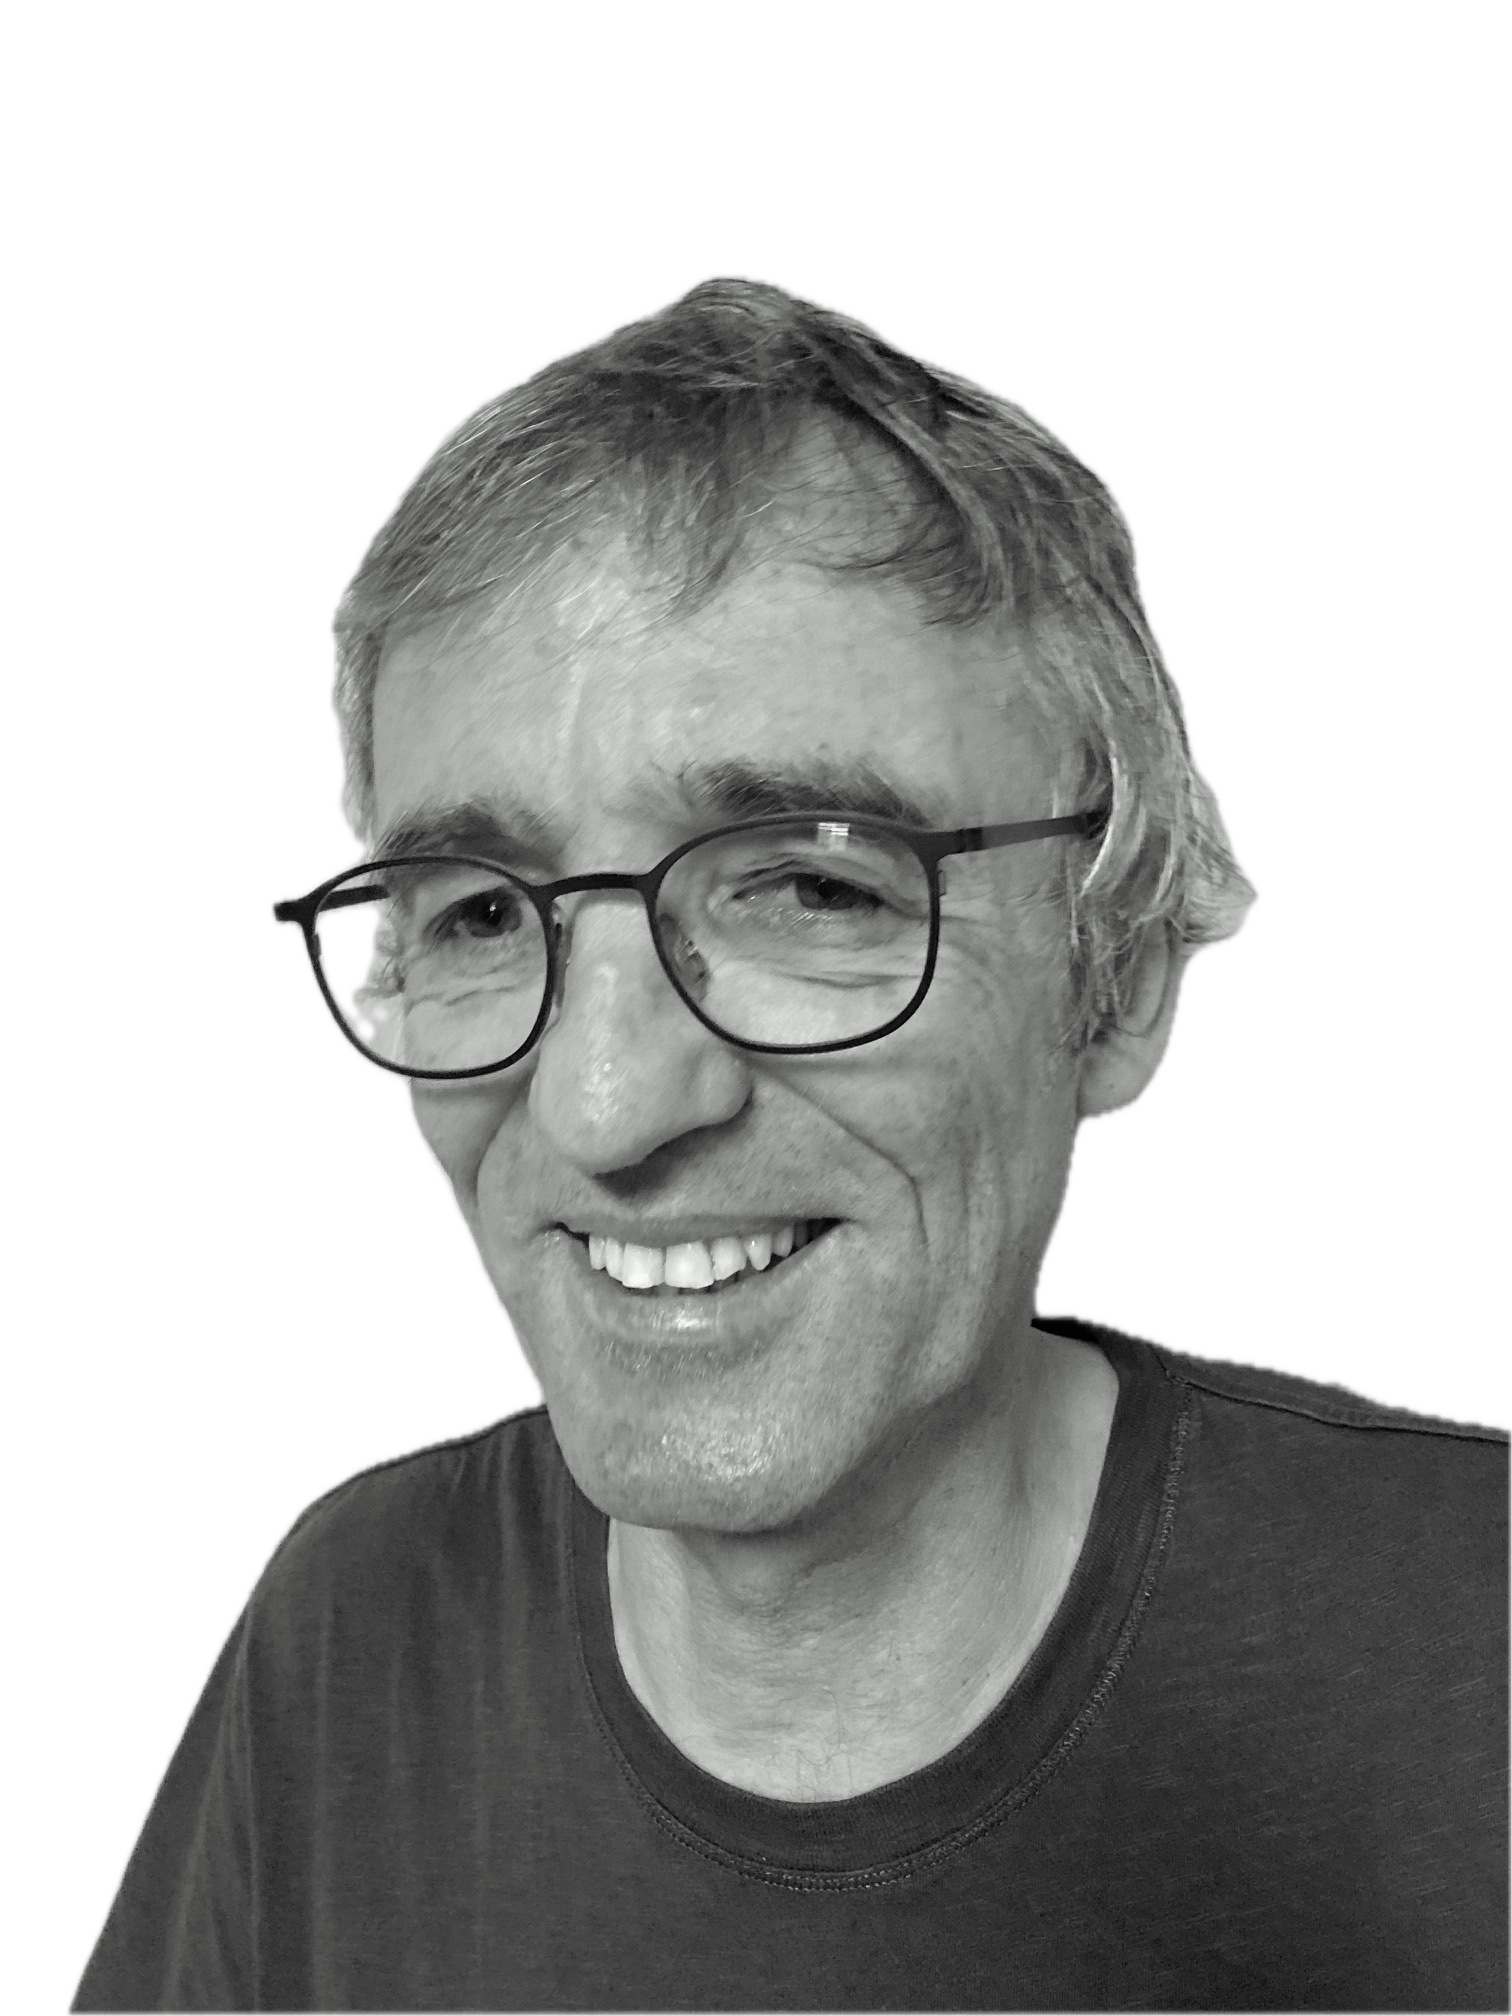
\includegraphics[width=1.20in]{test.png}};
		% \end{tikzpicture}
	
	% --- ISBN + Barcode unten rechts mit weißer Unterlage ---
	\begin{tikzpicture}[remember picture,overlay]
		\node[anchor=south east,
		xshift=-0.475in, yshift=-0.02in + 0.475in]
		at (current page.south east) {%
			\begin{tikzpicture}
				% Weiße Box als Unterlage (empfohlen ~2.00" x 1.20")
			%	\fill[white] (0,0) rectangle (2.00in,1.20in);
				% Barcode-Bild darauf platzieren (genaue Größe einhalten)
				\node[anchor=south west] at (0,0)
				{
\includegraphics[width=2.00in,height=1.20in]{barcode.png}};
			\end{tikzpicture}
		};
	\end{tikzpicture}
	
	% --- ISBN-Text neben/über dem Barcode (optional verschieben) ---
	
\begin{tikzpicture}[remember picture,overlay]
		\node[anchor=south east,
		xshift=-0.875in, yshift=1.25in + 0.475in] % etwas über der weißen Box
		at (current page.south east) {%
			{\sffamily\small\color{covertext} ISBN 978-3-912302-00-4}
		};
	\end{tikzpicture}
	
\end{document}
